%
% Tallinn University of Technology - bachelor, master thesis Éstonian template for LaTeX
%
%
% Public veresion 1.3
% 2023 translated main parts to Estonian (by Ago Luberg)
%
% Public version 1.2
% 2022 Updated by Karl Janson to match the new formatting guidelines
%
% Public Version 1.1
% 2019 Adjusted by Frank Korving for his Bachelor Thesis, with contributions from Sander Arnus
%
% Public version 1.0
% 2010 - 2013 Thijs Nugteren and Joos Buijs for Master Thesis
%
% THIS IS THE MAIN FILE (i.e. compile this file, compiling the others directly won't work)
%

\documentclass[12pt]{report} % Default font size is 12pt, default paper size is a4

% all the other includes etc. are done in the thesis.sty file.
\usepackage{thesis} % thesis formatting

%%%%%%%%%%%%%%%%%%%%%%%%%%%%%%%%%%%%%%%%%%%%%%%%%%%%%%%%%%%%%
% NOTE:                                                     %
%%%%%%%%%%%%%%%%%%%%%%%%%%%%%%%%%%%%%%%%%%%%%%%%%%%%%%%%%%%%%
% * Content chapter files are located in "chapters" folder, %
%   included using the "chapters_main.tex" file             %
%                                                           %
% * Appendices are located in "appendices" folder,          %
%   included using the "appendices_main.tex" file           %
%%%%%%%%%%%%%%%%%%%%%%%%%%%%%%%%%%%%%%%%%%%%%%%%%%%%%%%%%%%%%

%%%%%%%%%%%%%%%%%%%%%%%%%%%%%%%%%%%%%%%%%%%%%%%%%%%%%%%%%%%%%
% The commands below need to be defined.
% Square brackets should be removed.
% Estonian title page will be generated automatically       %
%%%%%%%%%%%%%%%%%%%%%%%%%%%%%%%%%%%%%%%%%%%%%%%%%%%%%%%%%%%%%

\newcommand{\lang}{Estonian} % Choose the language of the thesis (Estonian is the default one)

% If your work is in Estonian, English title is used for abstract. Don't forget to add it here!
% For English thesis is vice versa
\newcommand{\thesisTitleEng}{Thesis Title} % variable with thesis title
\newcommand{\thesisTitleEst}{Lõputöö pealkiri} % Title in Estonian

% Choose your thesis
\newcommand{\thesisType}{Master's Thesis}

% Thesis author
\newcommand{\authorName}{Kristjan Luik}
\newcommand{\studentcode}{211809IAPM}

% Second author. If you are the sole author, leave it as it is
\newcommand{\authorNameTwo}{[Second Author name]}
\newcommand{\studentcodeTwo}{[Student Code]}

% Third author. If you are the sole author, leave it as it is
\newcommand{\authorNameThree}{[Third Author name]}
\newcommand{\studentcodeThree}{[Student Code]}

% Main supervisor
\newcommand{\supervisorName}{Juhan-Peep Ernits}
\newcommand{\supervisortitle}{PhD}

% Co-supervisor. If you have only one supervisor, leave it as it is
\newcommand{\cosupervisorName}{[Co-Supervisor's Name]}
\newcommand{\cosupervisortitle}{[Academic degree]}

% Dates. Default to current current date.
% You can hard code a value by replacing the parameter with a text
% Year of publication (defaults to current year).
\newcommand{\Year}{\the\year{}}

% Signature date (defaults to today).
\newcommand{\signatureDate}{\ddmmyyyydate\today}

% PDF Metadata
\newcommand{\version}{0.1 version}
\newcommand{\keywords}{Important, comma, separated, keywords, applicable, to, your, thesis}

%%%%%%%%%%%%%%%%%%%%%%%%%%%%%%%%%%%%%%%%%%%%%%%%%%%%%%%%%%%%%
%            DO NOT EDIT BELOW THIS LINE                    %
%%%%%%%%%%%%%%%%%%%%%%%%%%%%%%%%%%%%%%%%%%%%%%%%%%%%%%%%%%%%%

\newcommand{\universityEng}{TALLINN UNIVERSITY OF TECHNOLOGY}
\newcommand{\schoolEng}{School of Information Technologies}
\newcommand{\universityEst}{TALLINNA TEHNIKAÜLIKOOL}
\newcommand{\schoolEst}{Infotehnoloogia teaduskond}

\ifthenelse {\equal{\authorName}{[Author name]}}
  {\newcommand{\authorNameEst}{[Ees- ja perenimi]}}
  {\newcommand{\authorNameEst}{\authorName}}

\ifthenelse {\equal{\studentcode}{[Student Code]}}
  {\newcommand{\studentcodeEst}{[Üliõpilaskood]}}
  {\newcommand{\studentcodeEst}{\studentcode}}

\ifthenelse {\equal{\supervisorName}{[Supervisor's Name]}}
  {\newcommand{\supervisorNameEst}{[Juhendaja nimi]}}
  {\newcommand{\supervisorNameEst}{\supervisorName}}

\ifthenelse {\equal{\supervisortitle}{[Academic degree]}}
  {\newcommand{\supervisortitleEst}{[Teaduskraad]}}
  {\newcommand{\supervisortitleEst}{\supervisortitle}}

\ifthenelse {\equal{\cosupervisorName}{[Co-Supervisor's Name]}}
  {\newcommand{\cosupervisorNameEst}{[Kaasjuhendaja nimi]}}
  {\newcommand{\cosupervisorNameEst}{\cosupervisorName}}

\ifthenelse {\equal{\cosupervisortitle}{[Academic degree]}}
  {\newcommand{\cosupervisortitleEst}{[Teaduskraad]}}
  {\newcommand{\cosupervisortitleEst}{\cosupervisortitle}}

\ifthenelse {\equal{\authorNameTwo}{[Second Author name]}}
  {\newcommand{\authorNameTwoEst}{[Teise autori nimi]}}
  {\newcommand{\authorNameTwoEst}{\authorNameTwo}}

\ifthenelse {\equal{\studentcodeTwo}{[Student Code]}}
  {\newcommand{\studentcodeTwoEst}{[Üliõpilaskood]}}
  {\newcommand{\studentcodeTwoEst}{\studentcodeTwo}}

\ifthenelse {\equal{\authorNameThree}{[Third Author name]}}
  {\newcommand{\authorNameThreeEst}{[Kolmanda autori nimi]}}
  {\newcommand{\authorNameThreeEst}{\authorNameThree}}

\ifthenelse {\equal{\studentcodeThree}{[Student Code]}}
  {\newcommand{\studentcodeThreeEst}{[Üliõpilaskood]}}
  {\newcommand{\studentcodeThreeEst}{\studentcodeThree}}

\ifthenelse {\equal{\thesisType}{Bachelor's Thesis}}
      {\newcommand{\thesisTypeEst}{Bakalaureusetöö}}
      {
        \ifthenelse {\equal{\thesisType}{Master's Thesis}}
          {\newcommand{\thesisTypeEst}{Magistritöö}}
          {\newcommand{\thesisTypeEst}{Bakalaureusetöö / Magistritöö}}
      }

\newcommand{\supervisor}{Supervisor}
\newcommand{\supervisorEst}{Juhendaja}

\newcommand{\cosupervisor}{Co-Supervisor}
\newcommand{\cosupervisorEst}{Kaasjuhendaja}


\ifthenelse{\not \equal{\lang}{ENG}}{
    % Estonian version
    \newcommand{\thesisTitle}{\thesisTitleEst}
    \newcommand{\abstractThesisTitle}{\thesisTitleEng}
    \newcommand{\langEst}{eesti}
    \newcommand{\langEng}{Estonian}
    \newcommand{\selectedLang}{estonian}
    \newcommand{\authorDeclarationTitle}{Autorideklaratsioon}
    \newcommand{\abstactTitle}{Annotatsioon}
    \newcommand{\secondAbstractTitle}{Abstract}
    \newcommand{\listOfTermsTitle}{Lühendite ja mõistete sõnastik}
    \newcommand{\tableOfContentsTitle}{Sisukord}
    \newcommand{\listOfFiguresTitle}{Jooniste loetelu}
    \newcommand{\listOfTablesTitle}{Tabelite loetelu}
    \newcommand{\referencesTitle}{Kasutatud kirjandus}
    \newcommand{\appendixTitle}{Lisa}
    \newcommand{\licenceTitle}{Lihtlitsents lõputöö reprodutseerimiseks ja lõputöö üldsusele kättesaadavaks tegemiseks}
    \newcommand{\licenceFootnote}{Lihtlitsents ei kehti juurdepääsupiirangu kehtivuse ajal vastavalt üliõpilase taotlusele lõputööle juurdepääsupiirangu kehtestamiseks, mis on allkirjastatud teaduskonna dekaani poolt, välja arvatud ülikooli õigus lõputööd reprodutseerida üksnes säilitamise eesmärgil. Kui lõputöö on loonud kaks või enam isikut oma ühise loomingulise tegevusega ning lõputöö kaas- või ühisautor(id) ei ole andnud lõputööd kaitsvale üliõpilasele kindlaksmääratud tähtajaks nõusolekut lõputöö reprodutseerimiseks ja avalikustamiseks vastavalt lihtlitsentsi punktidele 1.1. ja 1.2, siis lihtlitsents nimetatud tähtaja jooksul ei kehti.}
    \newcommand{\abstractPageNumber}{2}
  }{
    % English version
    \newcommand{\thesisTitle}{\thesisTitleEng}
    \newcommand{\abstractThesisTitle}{\thesisTitleEst}
    \newcommand{\langEst}{inglise}
    \newcommand{\langEng}{English}
    \newcommand{\selectedLang}{english}
    \newcommand{\authorDeclarationTitle}{Author’s declaration of originality}
    \newcommand{\abstactTitle}{Abstract}
    \newcommand{\secondAbstractTitle}{Annotatsioon}
    \newcommand{\listOfTermsTitle}{List of abbreviations and terms}
    \newcommand{\tableOfContentsTitle}{Table of contents}
    \newcommand{\listOfFiguresTitle}{List of figures}
    \newcommand{\listOfTablesTitle}{List of tables}
    \newcommand{\referencesTitle}{References}
    \newcommand{\appendixTitle}{Appendix}
    \newcommand{\licenceTitle}{Non-exclusive licence for reproduction and publication of a graduation thesis}
    \newcommand{\licenceFootnote}{The non-exclusive licence is not valid during the validity of access restriction indicated in the student's application for restriction on access to the graduation thesis that has been signed by the school's dean, except in case of the university's right to reproduce the thesis for preservation purposes only. If a graduation thesis is based on the joint creative activity of two or more persons and the co-author(s) has/have not granted, by the set deadline, the student defending his/her graduation thesis consent to reproduce and publish the graduation thesis in compliance with clauses 1.1 and 1.2 of the non-exclusive licence, the non-exclusive licence shall not be valid for the period.}
    \newcommand{\abstractPageNumber}{3}
  }

%
% PDF settings
%
\hypersetup
{
    pdfauthor={\authorName}, % Adds author's name in metadata, no need to change
    pdfsubject={\thesisTitle}, % Adds subject in metadata, no need to change
    pdfkeywords={\keywords} % Adds keywords in metadata
}

\begin{document}
\selectlanguage{\selectedLang}  % Translating automatically figure and table names (Figure / Joonis, Table / Tabel)

% Pages like title, auhtor's declaration, etc.
\ifthenelse{\equal{\lang}{ENG}}{
    % English TITLE PAGE
\begin{titlepage}
    \headheight = 57pt % This sets the height of the header
    \footskip = 5pt % This sets the distance between the bottom of the text area and the footer
    \headsep = 0pt % This sets the space between the header and the top of the main text
    
    \centering % Centers the content
    \universityEng\\ % University name variable
    \schoolEng % School name variable
    
    \vspace*{4.5 cm} % Adds vertical space between the top section and the next section of the title page
    
    \begin{center}
    
    % Adds authors names to the title page
    \authorName~ \studentcode \\
    \ifthenelse{\equal{\authorNameTwo}{[Second Author name]}}{}{\authorNameTwo\ \studentcodeTwo\\} % If the second author’s name is not provided, this line is ignored
    \ifthenelse{\equal{\authorNameThree}{[Third Author name]}}{}{\authorNameThree\ \studentcodeThree\\} % If the third author’s name is not provided, this line is ignored
    \vspace*{1.5 cm}
    
    \begin{Large}
        \fontsize{20}{16}{\textbf{\thesisTitleEng}}\\ % Adds thesis name to the title page
    \end{Large}
    
    \vspace*{1.5 cm}
    \thesisType   \\ % Adds thesis type to the title page
    \end{center}
    
    \vspace*{0.6 cm}
    
    \begin{flushright} % The following content will be aligned to the right
    % Adds supervisors to the title page
    \supervisor: \supervisorName\\ \supervisortitle\\
    \vspace*{0.2 cm}
    \ifthenelse{\equal{\cosupervisorName}{[Co-Supervisor's Name]}}{}{\cosupervisor: \cosupervisorName\\\cosupervisortitle} % If the cosupervisor’s name is not provided, this line is ignored
    \end{flushright}
    \vfill % Fills the remaining vertical space on the page, pushing any content below it to the bottom of the page
    
    Tallinn \Year % Adds city and year to the title page
    \end{titlepage}
}{}

% ESTONIAN TITLE PAGE
\begin{titlepage}
\headheight = 57pt % This sets the height of the header
\footskip = 5pt % This sets the distance between the bottom of the text area and the footer
\headsep = 0pt % This sets the space between the header and the top of the main text

\centering % Centers the content
\universityEst\\ % University name variable
\schoolEst % School name variable

\vspace*{4.5 cm} % Adds vertical space between the top section and the next section of the title page

\begin{center}

% Adds authors names to the title page
\authorNameEst~ \studentcodeEst \\
\ifthenelse{\equal{\authorNameTwoEst}{[Teise autori nimi]}}{}{\authorNameTwoEst\ \studentcodeTwoEst\\} % If the second author’s name is not provided, this line is ignored
\ifthenelse{\equal{\authorNameThreeEst}{[Kolmanda autori nimi]}}{}{\authorNameThreeEst\ \studentcodeThreeEst\\} % If the third author’s name is not provided, this line is ignored
\vspace*{1.5 cm}

\begin{Large}
    \fontsize{20}{16}{\textbf{\thesisTitleEst}}\\ % Adds thesis name to the title page
\end{Large}

\vspace*{1.5 cm}
\thesisTypeEst   \\ % Adds thesis type to the title page
\end{center}

\vspace*{0.6 cm}

\begin{flushright} % The following content will be aligned to the right
% Adds supervisors to the title page
\supervisorEst: \supervisorNameEst\\ \supervisortitleEst\\
\vspace*{0.2 cm}
\ifthenelse{\equal{\cosupervisorNameEst}{[Kaasjuhendaja nimi]}}{}{\cosupervisorEst: \cosupervisorNameEst\\\cosupervisortitleEst} % If the cosupervisor’s name is not provided, this line is ignored
\end{flushright}
\vfill % Fills the remaining vertical space on the page, pushing any content below it to the bottom of the page

Tallinn \Year % Adds city and year to the title page
\end{titlepage} % Includes the content from the file titlepage.tex located in the misc directory.

\pagenumbering{arabic}   % Sets the page numbering to Arabic numerals (1, 2, 3, ...). Purpose: To start normal page numbering in Arabic numerals after the title page.
\setcounter{page}{\abstractPageNumber} % Sets the current page number to 2.
\fontsize{12}{0} % This changes the font size to 12pt. The second number (0) usually specifies the line spacing, but here it is set to 0, which will be the default spacing.

\chapter*{\centerline{\authorDeclarationTitle}}\label{chapter:declaration} % This creates an unnumbered chapter titled "Autorideklaratsioon" and centers the text. The \label{chapter:declaration} creates a reference label for this chapter.
\ifthenelse{\equal{\lang}{ENG}}{
    \ifthenelse{\equal{\authorNameTwo}{[Second Author name]}}{ % If the second and the third authors are not provided
        I hereby certify that I am the sole author of this thesis and that this thesis has not been presented for examination or submitted for defense anywhere else. All used materials, references to the literature, and work of others have been cited.
        \begin{flushleft} %  The following content will be aligned to the left
            Author:~\authorName\\  % Author's name variable
    }{ % If the second and/or the third authors are provided
        We hereby certify that we are the sole authors of this thesis and that this thesis has not been presented for examination or submitted for defense anywhere else. All used materials, references to the literature, and work of others have been cited.
        \begin{flushleft}
            Authors:\ifthenelse{\equal{\authorNameThree}{[Third Author name]}}{ % Two authors
                \authorName~and~\authorNameTwo\\
            }{
                \authorName,~\authorNameTwo~and~\authorNameThree\\
            }
    }
}{
    \ifthenelse{\equal{\authorNameTwo}{[Second Author name]}}{ % If the second and the third authors are not provided
        Kinnitan, et olen koostanud antud lõputöö iseseisvalt ning seda ei ole kellegi teise poolt varem kaitsmisele esitatud. Kõik töö koostamisel kasutatud teiste autorite tööd, olulised seisukohad, kirjandusallikatest ja mujalt pärinevad andmed on töös viidatud.
        \begin{flushleft} %  The following content will be aligned to the left
            Autor:~\authorNameEst\\ % Author's name variable
    }{ % If the second and/or the third authors are provided
        Kinnitame, et oleme koostanud antud lõputöö iseseisvalt ning seda ei ole kellegi teise poolt varem kaitsmisele esitatud. Kõik töö koostamisel kasutatud teiste autorite tööd, olulised seisukohad, kirjandusallikatest ja mujalt pärinevad andmed on töös viidatud.
        \begin{flushleft}
            Autorid:\ifthenelse{\equal{\authorNameThree}{[Third Author name]}}{ % Two authors
                \authorName~ja~\authorNameTwo\\
            }{
                \authorName,~\authorNameTwo~ja~\authorNameThree\\
            }       
    }   
}

\vspace*{0.5cm}
\signatureDate % Date
\end{flushleft}
 % This inserts the content from the authordeclaration.tex file located in the misc folder.
\pagebreak % To move to the next page.

\chapter*{\centerline{\abstactTitle}}\label{chapter:abstract}
\ifthenelse{\equal{\lang}{ENG}}
    {Monitoring and accurately detecting forest logging activities is essential for sustainable forest management and environmental conservation. Traditional statistical approaches, such as Random Forest models applied to Sentinel-2 imagery, have shown promise but still suffer from limited spatial precision and require extensive manual post‑processing. In this thesis, we explore the efficacy of a self‑supervised Vision Transformer backbone, DINOv2, for few‑shot semantic segmentation of logging events in Sentinel‑2 multispectral images.

A smaller dataset comprising 100 clear‑cut polygons and their adjacent forest environs was constructed by integrating publicly available metsateatis records from the Estonian Forest Registry with Sentinel‑2 Level‑2A surface reflectance tiles. Initial geometric masks were refined through manual delineation and K‑Means clustering to differentiate coniferous and deciduous strata. The pretrained DINOv2 model was subsequently fine‑tuned on this dataset, utilizing the 10 m spatial resolution spectral bands alongside derived vegetation indices to enable pixel‑level discrimination of logging areas.

To evaluate performance, we compare the DINOv2‑based framework against benchmark Random Forest and U‑Net segmentation models, using Intersection over Union (IoU) and F1 score as primary metrics. This open-ended analysis will assess relative improvements in detection accuracy, annotation efficiency, and robustness to varying forest compositions. Further investigation will address temporal sequence incorporation and advanced cloud‑masking strategies.


% No need to change this
The thesis is in \langEng~and contains \calculatepages pages of text, 
\total{totalchapters} chapters\ifthenelse{\equal{\totvalue{figure}}{0}}{}{% If no figures, do nothing
, \total{figure} \ifnum\totvalue{figure}=1 figure\else figures\fi%
}\ifthenelse{\equal{\totvalue{table}}{0}}{}{% If no tables, do nothing
, \total{table} \ifnum\totvalue{table}=1 table\else tables\fi%
}.}
    {Metsavarade jätkusuutlikuks majandamiseks on hädavajalik metsaraiete tuvastamise täpsus ja ajakohasus. Traditsioonilised statistilised meetodid Sentinel‑2 multispektraalsete piltide töötlemisel on osutunud tõhusaks, kuid kannatavad sageli piiratud ruumilise eraldusvõime ja mahuka käsitöö tõttu. Käesolev uurimus käsitleb isejuhitud Vision Transformer’i peaahelat DINOv2 väheste õppeandmete põhist semantilist segmentatsiooni lageraie sündmuste tuvastamiseks.

Esmalt loodi andmestik, mis koosneb 100 lageraie polügoonist ja nende ümbritsevatest metsapiirkondadest. Nende põhjal ehitati programm, mis töötleb ja analüüsib metsateatisi, et luua geomeetrilised maskid, mis eristavad okas- ja lehtpuudega alasid. Lisaks sellele laeb programm alla Sentinel‑2 taseme 2A satelliidi pildid, et luua andmestik, mis sisaldab nii lageraie maske kui ka nende ümbritsevaid metsapiirkondi.

Tulemuste hindamiseks võrdleme DINOv2‑põhist raamistikku Random Foresti ja U‑Neti segmentatsioonimudelitega, kasutades peamiste kvaliteedimõõdikutena IoU‑d ja F1 skoori. Avatud lõpptulemite analüüs võimaldab hinnata tuvastustäpsuse, märgendamistõhususe ja mudeli robustsuse paranemist erinevates metsakoostistes. Edasistes uuringutes käsitletakse ajarealise analüüsi ja täiustatud pilvekatte maskimise strateegiaid.

% No need to change this
Lõputöö on kirjutatud \langEst~keeles ning sisaldab teksti \calculatepages leheküljel, 
\total{totalchapters} peatükki\ifthenelse{\equal{\totvalue{figure}}{0}}{}{% If no figures, do nothing
, \total{figure} \ifnum\totvalue{figure}=1 joonis\else joonist\fi%
}\ifthenelse{\equal{\totvalue{table}}{0}}{}{% If no tables, do nothing
, \total{table} \ifnum\totvalue{table}=1 tabel\else tabelit\fi%
}.}
\pagebreak

\chapter*{\begin{center}
    {\secondAbstractTitle}\\[12pt] % Adds a 12pt space below \secondAbstractTitle
    \abstractThesisTitle
\end{center}}\label{chapter:abstract-english}
\ifthenelse{\equal{\lang}{ENG}}
    {Metsavarade jätkusuutlikuks majandamiseks on hädavajalik metsaraiete tuvastamise täpsus ja ajakohasus. Traditsioonilised statistilised meetodid Sentinel‑2 multispektraalsete piltide töötlemisel on osutunud tõhusaks, kuid kannatavad sageli piiratud ruumilise eraldusvõime ja mahuka käsitöö tõttu. Käesolev uurimus käsitleb isejuhitud Vision Transformer’i peaahelat DINOv2 väheste õppeandmete põhist semantilist segmentatsiooni lageraie sündmuste tuvastamiseks.

Esmalt loodi andmestik, mis koosneb 100 lageraie polügoonist ja nende ümbritsevatest metsapiirkondadest. Nende põhjal ehitati programm, mis töötleb ja analüüsib metsateatisi, et luua geomeetrilised maskid, mis eristavad okas- ja lehtpuudega alasid. Lisaks sellele laeb programm alla Sentinel‑2 taseme 2A satelliidi pildid, et luua andmestik, mis sisaldab nii lageraie maske kui ka nende ümbritsevaid metsapiirkondi.

Tulemuste hindamiseks võrdleme DINOv2‑põhist raamistikku Random Foresti ja U‑Neti segmentatsioonimudelitega, kasutades peamiste kvaliteedimõõdikutena IoU‑d ja F1 skoori. Avatud lõpptulemite analüüs võimaldab hinnata tuvastustäpsuse, märgendamistõhususe ja mudeli robustsuse paranemist erinevates metsakoostistes. Edasistes uuringutes käsitletakse ajarealise analüüsi ja täiustatud pilvekatte maskimise strateegiaid.

% No need to change this
Lõputöö on kirjutatud \langEst~keeles ning sisaldab teksti \calculatepages leheküljel, 
\total{totalchapters} peatükki\ifthenelse{\equal{\totvalue{figure}}{0}}{}{% If no figures, do nothing
, \total{figure} \ifnum\totvalue{figure}=1 joonis\else joonist\fi%
}\ifthenelse{\equal{\totvalue{table}}{0}}{}{% If no tables, do nothing
, \total{table} \ifnum\totvalue{table}=1 tabel\else tabelit\fi%
}.}
    {Monitoring and accurately detecting forest logging activities is essential for sustainable forest management and environmental conservation. Traditional statistical approaches, such as Random Forest models applied to Sentinel-2 imagery, have shown promise but still suffer from limited spatial precision and require extensive manual post‑processing. In this thesis, we explore the efficacy of a self‑supervised Vision Transformer backbone, DINOv2, for few‑shot semantic segmentation of logging events in Sentinel‑2 multispectral images.

A smaller dataset comprising 100 clear‑cut polygons and their adjacent forest environs was constructed by integrating publicly available metsateatis records from the Estonian Forest Registry with Sentinel‑2 Level‑2A surface reflectance tiles. Initial geometric masks were refined through manual delineation and K‑Means clustering to differentiate coniferous and deciduous strata. The pretrained DINOv2 model was subsequently fine‑tuned on this dataset, utilizing the 10 m spatial resolution spectral bands alongside derived vegetation indices to enable pixel‑level discrimination of logging areas.

To evaluate performance, we compare the DINOv2‑based framework against benchmark Random Forest and U‑Net segmentation models, using Intersection over Union (IoU) and F1 score as primary metrics. This open-ended analysis will assess relative improvements in detection accuracy, annotation efficiency, and robustness to varying forest compositions. Further investigation will address temporal sequence incorporation and advanced cloud‑masking strategies.


% No need to change this
The thesis is in \langEng~and contains \calculatepages pages of text, 
\total{totalchapters} chapters\ifthenelse{\equal{\totvalue{figure}}{0}}{}{% If no figures, do nothing
, \total{figure} \ifnum\totvalue{figure}=1 figure\else figures\fi%
}\ifthenelse{\equal{\totvalue{table}}{0}}{}{% If no tables, do nothing
, \total{table} \ifnum\totvalue{table}=1 table\else tables\fi%
}.}
\pagebreak

\chapter*{\centerline{\listOfTermsTitle}}\label{chapter:terms}
\begin{longtable}{p{3cm}p{10cm}}  % Begins a longtable environment. The 'p{3cm}' and 'p{10cm}' specify column widths.
Ülelennu sagedus & (\textit{Revisit time}) ajavahemik, mis jääb mingi kindla
piirkonna satelliidivaatluste vahele\\
Lainepikkus & (\textit{Band}) lainepikkuste vahemik elektromagnetkiirguse spektris \\
peaahel & (\textit{Backbone}) mudeli peamine arhitektuur, mis on eelnevalt treenitud
ja millele on lisatud täiendavad kihid, et saavutada soovitud ülesanne\\
R2 & R-ruut (\textit{R-squared}) regressioonimudeli täpsuse mõõdik, mis näitab
mudeli selgitusvõimet andmete variatsioonis\\
IoU & Ühenduse indeks (\textit{Intersection over Union}) mõõdik, mis hindab
mudeli täpsust, võrreldes ennustatud ja tegelikke tulemusi\\
F1 skoor & F1 skoor (\textit{F1 score}) mõõdik, mis ühendab täpsuse ja
meeldetuletuse ja annab tasakaalustatud hinnangu mudeli jõudlusele\\
NDVI & Taimede indeksi (\textit{Normalized Difference Vegetation Index}) mõõdik, mis
hindab taimekatte tihedust ja elujõudlust, arvutatakse punase ja lähedase
infrapunase lainepikkuse vahekorra põhjal\\
Jääkühik & Jääkühikud (\textit{residual blocks}) on närvivõrgu arhitektuurimuster, kus konvolutsioonikihide jadale lisatakse sisendi ja väljundi vahe (residuaal) skip-ühenduse kaudu, et hõlbustada sügavate võrkude treenimist ja vältida gradientide kadu. \\
DICE & DICE (\textit{Dice coefficient}) on mõõdik, mis hindab segmentatsiooni \\
CrossEntropyLoss & Rist-entsentratsiooni kadu (\textit{Cross Entropy Loss}) on
tüüpiline kadufunktsioon klassifitseerimisülesannetes, mis mõõdab erinevust mudeli ennustatud tõenäosuste ja tegelike klasside vahel. \\
Ülesobitamine & Ülesobitamine (\textit{overfitting})  on nähtus, kus mudel õpib treeningandmeid liiga hästi, sealhulgas müra ja ebaolulisi mustreid, mis viib halvenenud üldistumisvõimele uute andmete puhul. See võib põhjustada kõrgeid treeningtulemusi, kuid madalaid valideerimistulemusi. \\
\end{longtable}
\addtocounter{table}{-1} % Decreases the table counter by 1 so that it doesn't increment the table number in the document

\pagebreak

\phantomsection % This creates a linkable section for hyperref without placing visible content.
\setcounter{tocdepth}{2} % Sets maximum depth of Table Of Contents. A value of 2 includes sections and subsections.
\renewcommand{\contentsname}{\tableOfContentsTitle} % This renames the table of contents heading to "Sisukord" (Estonian for "Table of Contents").
\tableofcontents % This generates the table of contents for the document.

% If you don't have any figures, remove the next block of code
\clearpage \phantomsection % This forces a new page and creates an invisible section for hyperlinking.
\setcounter{figure}{0} % To start the figure numbering afresh from 1 in the subsequent section.
\renewcommand{\listfigurename}{\listOfFiguresTitle}
\listoffigures % This generates the list of figures for the document.

% If you don't have any tables, remove the next block of code
\clearpage \phantomsection
\renewcommand{\listtablename}{\listOfTablesTitle}
\listoftables % This generates the list of tables for the document.


% Content chapters
\zlabel{firstpagetocount}       % DO NOT REMOVE! Used for counting number of pages of main text

% Part Labels Explanation:
% Labels in the form \label{chapter:<part_name>} are used to categorize chapters into specific parts of the thesis structure.
% These labels are essential for calculating the ratio of text dedicated to different thesis sections (e.g., Introduction, Methodology, Results, Discussion, Summary).
% Allowed labels:
% - chapter:introduction -> Introduction (<10% of the text).
% - chapter:method       -> Methodology (<20% of the text).
% - chapter:results      -> Results (30–40% of the text).
% - chapter:discussion   -> Analysis, Discussion, and Conclusions (30–40% of the text).
% - chapter:summary      -> Summary (<0.5 pages).
% How to use: Add a \label{chapter:<part_name>} for each chapter to indicate its part. 
% These labels ensure consistency and allow automated tests to validate the thesis structure.

\chapter{Introduction}\label{chapter:introduction} % This command creates a numbered chapter titled "Sissejuhatus" (Estonian for "Introduction"). The \label{chapter:introduction} assigns a label to the chapter, allowing you to reference it later (e.g., \ref{chapter:introduction}).
Some basic ways to manipulate text are \textit{italics} and \textbf{bold}. 

One can reference Figures (see Figure \ref{fig:taltech} for example) as well as cite references which are defined in the \textit{references.bib} file \cite{spectre}, \cite{example-reference} .

\begin{figure}[hb] % h-here, if possible; H-here, definitely; t-top of the page; b-bottom of the page; p-page of floats
    \centering
    
\includegraphics[width=.3\textwidth]{figures/taltech.jpg} % Includes an image from the specified path, setting the width to 50% of the text width
    \caption{An image of TalTech logo.} % Provides a caption for the figure, italicizing the text
    \label{fig:taltech} % Sets a label for the figure to be referenced later
\end{figure}

The \textit{Bibliography}, \textit{List of Figures}, and \textit{List of Tables} are automatically\cite{prittSatelliteImageClassification2017} generated\cite{prittSatelliteImageClassification2017}, with references, figures, and tables updated as needed\cite{prittSatelliteImageClassification2017}. Unused citations won't appear, and numbering follows the order of appearance.
One can create an itemized list:
\begin{itemize}  % Begins an itemized list environment
    \item item a  % First item in the list
    \item item b  % Second item in the list...
    \item ...
\end{itemize}

Or enumerate them:
\begin{enumerate} % Begins an enumerated list environment
    \item item x  % First item in the list...
    \item item y
    \item ...
\end{enumerate}


A pair of side-by-side images can be seen in Figure \ref{fig:sidebyside}. Each image can also be referenced individually; for instance, refer to Figure \ref{fig:tux1} for the first image.

\begin{figure}[htb] % Placement specifier: h-here, t-top, b-bottom
    \centering
    % First subfigure
    \begin{subfigure}[b]{0.3\textwidth} % Set width for side-by-side arrangement
        
\includegraphics[width=\textwidth]{figures/penguins/tux1.png} % Image path and full width in subfigure
        \caption{} % Leave caption empty to automatically label this subfigure as (a)
        \label{fig:tux1}
    \end{subfigure}
    % Second subfigure
    \begin{subfigure}[b]{0.3\textwidth} % Set width for side-by-side arrangement
        
\includegraphics[width=\textwidth]{figures/penguins/tux2.png} % Path and full width in subfigure
        \caption{} % Leave caption empty to automatically label this subfigure as (b)
    \end{subfigure}
    
    \caption{Side-by-side images of Tux: (a) on a white background, (b) on a black background.} % Main caption for the whole figure environment
    \label{fig:sidebyside} % Main label to reference the entire figure
\end{figure}

\subsubsection{Using Part Labels}
Labels in the format \texttt{\textbackslash label\{chapter:<part\_name>\}} are used to categorize chapters into specific parts of the thesis structure. They play an important role in maintaining the document's structure and validating its compliance with expected ratios for each section.

\begin{itemize}
    \item \textbf{Allowed Labels:}
        \begin{itemize}
            \item \texttt{chapter:introduction} - For the \textbf{Introduction} section (less than 10\% of the thesis).
            \item \texttt{chapter:method} - For the \textbf{Methodology} section (up to 20\%).
            \item \texttt{chapter:results} - For the \textbf{Results} section (30–40\%).
            \item \texttt{chapter:discussion} - For the \textbf{Discussion and Analysis} section (30–40\%).
            \item \texttt{chapter:summary} - For the \textbf{Summary} section (less than 0.5 pages).
        \end{itemize}
    \item \textbf{Purpose:} These labels enable automated tools to check if each part of your thesis conforms to the required word count ratios.
    \item \textbf{Usage:} Add the appropriate label to the \texttt{\textbackslash chapter} command for each chapter in your document.
    \item \textbf{Subdividing a Part into Multiple Chapters:} If a single part (e.g., \textbf{Discussion}) is split into multiple chapters, ensure the main part label remains consistent, and additional identifiers can be appended to distinguish chapters. For instance:
        \begin{itemize}
            \item \texttt{\textbackslash label\{chapter:discussion-analysis\}} for an analysis chapter.
            \item \texttt{\textbackslash label\{chapter:discussion-discussion\}} for the primary discussion.
            \item \texttt{\textbackslash label\{chapter:discussion-conclusions\}} for conclusions.
        \end{itemize}
        Only the main part (e.g., \texttt{chapter:discussion}) is relevant for validation and ratio calculations; the suffixes (e.g., \texttt{-analysis}, \texttt{-discussion}, \texttt{-conclusions}) are for your internal organization and clarity.
\end{itemize}

% \blindtext % generates placeholder text. Uncomment to add text before the table if you'd like to see how it continues across pages.

Here, you can use \textbackslash blindtext to see how the table continues on the next page.  This command generates dummy text that can help you visualize the layout of your document. Uncomment the line above to add filler text.

A table with three columns can be seen in Table \ref{tab:requirements}.
\begin{longtable}[hp]{|p{0,5cm}|p{10cm}|p{3cm}|} % Begins a longtable with three columns, defining specific widths for each column
	\caption{A table with some requirements.} % Provides a caption for the table, italicizing the text
	\label{tab:requirements}\\ \hline % Sets a label for the table and starts the table with a horizontal line
	\textbf{Nr} &  \textbf{Requirement} & \textbf{Weight}  \\ % Table header with bold text
	\hline % Adds a horizontal line after the header
	\endfirsthead % Marks the end of the header for the first page of the table
	\multicolumn{3}{l} % Merges three columns for the continuation note
	{\tablename\ \thetable\ -- \textit{Continues...}} \\ % Creates a continuation note with italicized text
	\hline
	\textbf{Nr} &  \textbf{Requirement} & \textbf{Weight}  \\ % Table header for continued pages, with bold text
	\hline
	\endhead % Marks the end of the header for all pages after the first
	\hline \multicolumn{3}{l}{\textit{Continues...}} \\ % Adds a note at the end of the table for continued pages
	\endfoot % Marks the end of the table body
	\hline
	\endlastfoot % Marks the end of the table for the last page
1 & Price & High\\ \hline % First row of the table with data and a horizontal line...
2 & Variety& Middle\\ \hline
3 & Support& Low\\ \hline
\end{longtable}

We can use variables set in the \textit{main.tex} file to render values like our title (\thesisTitleEng) or supervisor names (\textbf{Supervisor}: \supervisorName, \textbf{Co-supervisor}: \cosupervisorName ). %  This command inserts the content from the file introduction.tex located in the chapters folder.

\chapter{First Chapter}\label{chapter:method}
This is the first real chapter of this thesis. Other chapters can be easily referenced, for example the introduction can be found as Chapter \ref{chapter:introduction}. Sections and/or subsections need to be labeled before one can reference them. See Section \ref{sec:second-section} for an example.

\section{First Section of the First Chapter} % This creates a new section with the title "First Section of the First Chapter."
Some text in the first section. %  This is regular text content inside the section.
\subsection{First Subsection} %This creates a new subsection titled "First Subsection."
As well as some text in this subsection. 
\subsubsection{First Subsubsection} % This creates a subsubsection titled "First Subsubsection."
The Table of Contents only goes 3 layers deep (Chapter - Section - Subsection) so this subsubsection is not seen there.

\section{Second Section of the First Chapter}\label{sec:second-section} % This creates a new section titled "Second Section of the First Chapter" and assigns the label sec:second-section.The label allows for internal referencing to this section elsewhere in the document. 


\chapter{Second Chapter}\label{chapter:results}
One of the best resources for \LaTeX~ basics, and advanced constructs, is the \LaTeX~ wikibook\footnote{To be found at~\url{http://en.wikibooks.org/wiki/LaTeX/}}. Of course fellow students, colleagues and a good internet search using your favorite search engine can do wonders if you're stuck. 

\chapter{Third Chapter}\label{chapter:discussion}
third

\chapter{Summary}\label{chapter:summary} 
summ

\zlabel{lastpagetocount}        % DO NOT REMOVE! Used for counting number of pages of main text


\pagebreak % Content that follows starts on the new page
\phantomsection % Creates linkable section without placing visible content
\addcontentsline{toc}{chapter}{\referencesTitle} % adds a new chapter entry labeled "Kasutatud kirjandus" to TOC
\printbibliography[title=\referencesTitle] % The command pulls from the .bib file and and formats the output

\pagebreak
\phantomsection
\appendix % This command signals that the following sections will be appendices.

% \addcontentsline{toc}{chapter}{Appendices}
% \chapter*{Appendices}
\renewcommand{\thechapter}{\arabic{chapter}} % This command redefines how chapter numbers are displayed.

% Licence
% Footnote for a licence
% This command adds an entry to the table of contents (TOC).
\addcontentsline{toc}{chapter}{\appendixTitle~1 -- \licenceTitle}\label{chapter:licence}

% This is the title of the licence section, which is being displayed as a chapter heading and it adds a footnote at the end of the chapter title
{\let\clearpage\relax\chapter*{\appendixTitle~1 -- \licenceTitle\footnote{\licenceFootnote}}}
% Generates the list of supervisors. Do not edit
\newcommand{\supervisorList}[1]
{
  \ifthenelse{\equal{#1}{[Co-Supervisor's Name]}}{\mbox{\supervisorName}}{\mbox{\supervisorName}~and \mbox{\cosupervisorName}}
}

\newcommand{\supervisorListEst}[1]
{
  \ifthenelse{\equal{#1}{[Kaasjuhendaja nimi]}}{\mbox{\supervisorNameEst}}{\mbox{\supervisorNameEst}~and \mbox{\cosupervisorNameEst}}
}

% The licence should be automatically filled, please double check that everything is fine before submitting
\ifthenelse{\equal{\lang}{ENG}}{
  \ifthenelse{\equal{\authorNameTwo}{[Second Author name]}}
  {
  I \authorName

  \begin{enumerate}[label*=\arabic*.]
      \item Grant Tallinn University of Technology free licence (non-exclusive licence) for my thesis ``\thesisTitleEng'', supervised by \supervisorList{\cosupervisorName}
      \begin{enumerate}[label*=\arabic*.]
          \item to be reproduced for the purposes of preservation and electronic publication of the graduation thesis, incl. to be entered in the digital collection of the library of Tallinn University of Technology until expiry of the term of copyright;
          \item to be published via the web of Tallinn University of Technology, incl. to be entered in the digital collection of the library of Tallinn University of Technology until expiry of the term of copyright
      \end{enumerate}
      \item I am aware that the author also retains the rights specified in clause 1 of the nonexclusive licence.
      \item I confirm that granting the non-exclusive licence does not infringe other persons' intellectual property rights, the rights arising from the Personal Data Protection Act or rights arising from other legislation.
  \end{enumerate}
  }
  {
    We\ifthenelse{\equal{\authorNameThree}{[Third Author name]}}{ % Two authors
          \authorName~and~\authorNameTwo
        }{
          \authorName,~\authorNameTwo~and~\authorNameThree
        }

    \begin{enumerate}[label*=\arabic*.]
        \item Grant Tallinn University of Technology free licence (non-exclusive licence) for our thesis ``\thesisTitleEng'', supervised by \supervisorList{\cosupervisorName}
        \begin{enumerate}[label*=\arabic*.]
            \item to be reproduced for the purposes of preservation and electronic publication of the graduation thesis, incl. to be entered in the digital collection of the library of Tallinn University of Technology until expiry of the term of copyright;
            \item to be published via the web of Tallinn University of Technology, incl. to be entered in the digital collection of the library of Tallinn University of Technology until expiry of the term of copyright
        \end{enumerate}
        \item We are aware that the authors also retain the rights specified in clause 1 of the nonexclusive licence.
        \item We confirm that granting the non-exclusive licence does not infringe other persons' intellectual property rights, the rights arising from the Personal Data Protection Act or rights arising from other legislation.
    \end{enumerate}
  }
} {
  \ifthenelse{\equal{\authorNameTwo}{[Second Author name]}}
  {
    Mina, \authorNameEst

    \begin{enumerate}[label*=\arabic*.]
        \item Annan Tallinna Tehnikaülikoolile tasuta loa (lihtlitsentsi) enda loodud teose ``\thesisTitleEst'', mille juhendaja on \supervisorListEst{\cosupervisorNameEst}
        \begin{enumerate}[label*=\arabic*.]
            \item reprodutseerimiseks lõputöö säilitamise ja elektroonse avaldamise eesmärgil, sh Tallinna Tehnikaülikooli raamatukogu digikogusse lisamise eesmärgil kuni autoriõiguse kehtivuse tähtaja lõppemiseni;
            \item üldsusele kättesaadavaks tegemiseks Tallinna Tehnikaülikooli veebikeskkonna kaudu, sealhulgas Tallinna Tehnikaülikooli raamatukogu digikogu kaudu kuni autoriõiguse kehtivuse tähtaja lõppemiseni.
        \end{enumerate}
        \item Olen teadlik, et käesoleva lihtlitsentsi punktis 1 nimetatud õigused jäävad alles ka autorile.
        \item Kinnitan, et lihtlitsentsi andmisega ei rikuta teiste isikute intellektuaalomandi ega isikuandmete kaitse seadusest ning muudest õigusaktidest tulenevaid õigusi.
    \end{enumerate}
  }
  {
    Meie,\ifthenelse{\equal{\authorNameThree}{[Third Author name]}}{ % Two authors
              \authorName~ja~\authorNameTwo
          }{
              \authorName,~\authorNameTwo~ja~\authorNameThree
          }       

    \begin{enumerate}[label*=\arabic*.]
        \item Anname Tallinna Tehnikaülikoolile tasuta loa (lihtlitsentsi) enda loodud teose ``\thesisTitleEst'', mille juhendaja on \supervisorListEst{\cosupervisorNameEst}
        \begin{enumerate}[label*=\arabic*.]
            \item reprodutseerimiseks lõputöö säilitamise ja elektroonse avaldamise eesmärgil, sh Tallinna Tehnikaülikooli raamatukogu digikogusse lisamise eesmärgil kuni autoriõiguse kehtivuse tähtaja lõppemiseni;
            \item üldsusele kättesaadavaks tegemiseks Tallinna Tehnikaülikooli veebikeskkonna kaudu, sealhulgas Tallinna Tehnikaülikooli raamatukogu digikogu kaudu kuni autoriõiguse kehtivuse tähtaja lõppemiseni.
        \end{enumerate}
        \item Oleme teadlikud, et käesoleva lihtlitsentsi punktis 1 nimetatud õigused jäävad alles ka autoritele.
        \item Kinnitame, et lihtlitsentsi andmisega ei rikuta teiste isikute intellektuaalomandi ega isikuandmete kaitse seadusest ning muudest õigusaktidest tulenevaid õigusi.
    \end{enumerate}
  }
}

% Defaults to current date. If you want a specific date, replace \signaturedate with hardcoded value
\signatureDate
 % This command imports the content from an external file

% Other appendices
% NOTE: Appendix 1 is always the non-exclusive licence.
% Therefore, your appendices need to start from 2.

\clearpage % Forces a page break, ending the current page and starting a new one

\addcontentsline{toc}{chapter}{\appendixTitle~2 -- Vektor maskide loomine kasutades QGISi}\label{chapter:appendix-vektor-maskide-loomine}
\chapter*{\appendixTitle~2 -- Vektor maskide loomine kasutades QGISi}
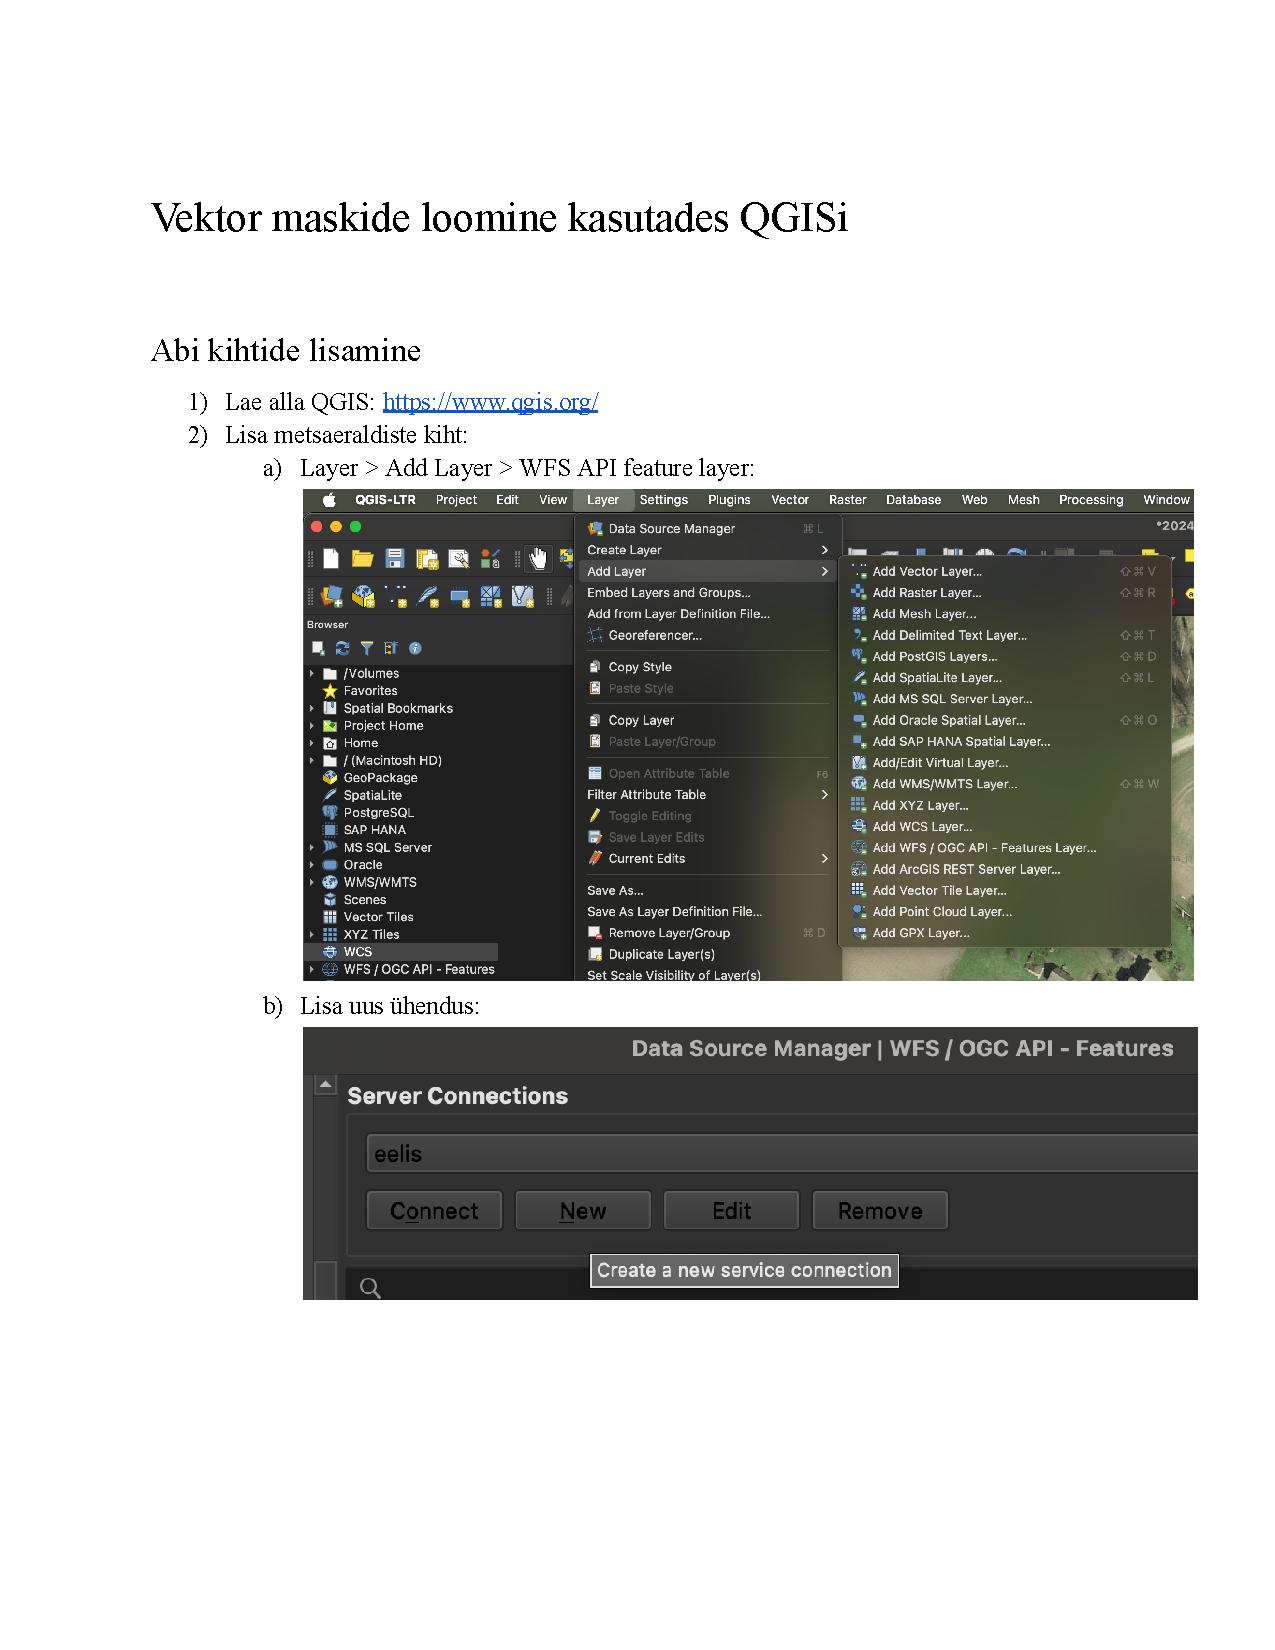
\includepdf[pages=-]{appendices/Vektor_maskide_loomine_kasutades_QGISi.pdf}


\end{document}
